\documentclass[12pt]{iopart}

\newcommand{\gguide}{{\it Preparing graphics for IOP Publishing journals}}
\usepackage{iopams}  

\usepackage{booktabs}
\usepackage{parskip}
\usepackage{graphicx}
\usepackage{multirow}
% \usepackage{mathtools}
\usepackage[capitalise]{cleveref}
\Crefname{equation}{Eq.}{Eqs.}
\Crefname{figure}{Fig.}{Figs.}
\Crefname{tabular}{Tab.}{Tabs.}
\Crefname{section}{Sec.}{Secs.}

\begin{document}

\title[Quantum Feature Space of Qubit in Arbitrary Bath]{Quantum Feature Space of Qubit in Arbitrary Bath}

\author{Chris Wise$^{1,*}$, Akram Youssry$^{2}$, Alberto Peruzzo$^{2,3}$, Jo Plested$^{1}$, and Matt Woolley$^4$}

\address{$^1$School of Systems and Computing, University of New South Wales, Canberra, ACT, 2601, Australia}
\address{$^2$Quantum Photonics Laboratory and Centre for Quantum Computation and Communication Technology, RMIT University, Melbourne, VIC 3000, Australia}
\address{$^3$Qubit Pharmaceuticals, Advanced Research Department, Paris, France}
\address{$^4$Centre for Engineered Quantum Systems, University of New South Wales, Canberra, ACT, 2601, Australia}
\address{$^*$Author to whom any correspondence should be addressed.}
\ead{c.wise@unswalumni.com}

\begin{abstract}
    Qubit control protocols have traditionally leveraged a characterisation of the qubit-bath coupling via its power spectral density. Previous work suggested inferring noise operators that characterise the influence of a classical bath using a neural network-based approach. Here, we show that no expensive neural networks are needed, and this noise operator description admits an efficient parameterisation. We refer to this parametrisation as the \textit{quantum feature space} of the qubit dynamics resulting from noise arising from the coupled bath. We show that the Euclidean distance defined over the quantum feature space provides an effective method for classifying noise processes in the presence of a given set of controls. We demonstrate a simple random forest algorithm's effectiveness in classifying the stationarity and broad class of noise processes perturbing a qubit, with the input being the quantum feature space. Finally, we explore how control pulse parameters map to the quantum feature space.
\end{abstract}

\vspace{2pc}
\noindent{\it Keywords}:  quantum control, quantum features, classification, clustering

\section{Introduction}
Noise in quantum computers resulting in qubits losing coherence (decoherence) is due to unwanted bath coupling~\cite{bravyi2018correcting}. One way to mitigate decoherence is to decouple the qubit from the bath by applying a control field, a technique known as dynamical decoupling and is implemented as a series of pulses~\cite{viola1999dynamical}.

Control pulses to decouple quantum systems from baths were first studied in nuclear magnetic resonance imaging~\cite{degen2017quantum, boss2016one}, and their use to address decoherence is known as dynamical decoupling. Within this framework, control pulses are applied for a time $\tau$ and then turned off for time $\tau$, and this pattern is repeated $N$ times. This oscillating pulse sequence design is the Carr-Purcell-Meiboom-Gill (CPMG) sequence~\cite{carr1954effects, meiboom1958modified}.

\'Alvarez and Suter (AS) proposed a modified CPMG sequence to perform qubit spectroscopy~\cite{alvarez2011measuring}. AS pulses are part of a family of pulses used for so-called dynamical decoupling noise spectroscopy, and they measure qubit coherence as a function of time.

This empirical coherence data, obtained by AS pulses, for example, is fitted to theoretical coherence curves corresponding to parametric noise spectra~\cite{von2020two, sun2022self}. However, this method requires an accurate model of system dynamics~\cite{wise2021using}, which can be challenging to develop in general~\cite{martina2021machine}. Further, if an inappropriate parametric noise spectrum is chosen \textit{a priori}, the estimated noise spectrum is an inappropriate model of system dynamics and subsequently, control pulses optimised using this system model will likely be ineffective~\cite{martina2021machine}.

More direct methods of noise spectroscopy include techniques like two-point correlation, which measures the correlation function of the noise by implementing gates at different times and measuring the change in the qubit state~\cite{baroni2022nuclear}. The Fourier transform of this correlation function gives the noise spectrum. However, this method can be resource-intensive, time-consuming, computationally expensive and requires the noise to be stationary~\cite{von2020two,wise2021using,martina2023deep,vezvaee2022noise}.

The authors of~\cite{vezvaee2022noise} developed a quantum noise spectroscopy method that used the Fourier transform of free induction decay measurements of coherence curves. The method accurately recovered the correct noise spectra and outperformed previous decoupling schemes while significantly reducing experimental overhead. However, the method makes several assumptions that limit the work's applicability. For example, the authors assume the qubit is only subject to dephasing, where the qubit thermal relaxation process occurs over a much longer time scale than phase randomisation, and that the frequency fluctuations of a qubit are subject to stationary zero-mean Gaussian noise.

In~\cite{wise2021using}, researchers instead used deep learning techniques to infer accurate qubit noise spectra. The technique used coherence curves as input to a recurrent neural network with a feedforward neural network head to estimate the noise spectrum. They showed that the model could accurately estimate the qubit noise spectrum using only the coherence curves and outperformed the standard noise spectroscopy techniques.

Researchers in~\cite{martina2023deep} further demonstrated the effectiveness of deep learning by using it to reconstruct the PSD of an ensemble of carbon impurities around a diamond's nitrogen-vacancy centre.

Youssry et al.~\cite{youssry2020characterization} introduced a grey-box model separating control and system-bath dynamics. In this work, time-dependent Hamiltonians and unitaries specified the control dynamics, and a form of recurrent neural network (a gated recurrent unit) was used to predict the system-bath dynamics associated with control pulses.

The input to this GRU was parameterised control pulses as a sequence of vectors. The model output was the parameterisation of a noise operator. The authors showed that the grey-box model could be used for qubit control pulse optimisation and qubit noise spectroscopy. The formalism used in this work is discussed in greater detail in~\cref{sec:noise_operator_formalism}.

The grey-box model approach was subsequently used for qubit control optimisation in the presence of a non-Markovian bath~\cite{youssry2022multi}.

Despite the success of~\cite{wise2021using,martina2023deep,youssry2020characterization,youssry2022multi}, these approaches are limited by their use of deep learning models, specifically the expense of training deep learning models and the need for large datasets. Expensive models are undesirable as noise processes in quantum systems can drift over time~\cite{seedhouse2023spatio,nakamura2024gate}, necessitating new training data and model retraining potentially daily or even hourly. Additionally, noise profiles may change from one physical qubit to another~\cite {sung2019non}, so a specific model may be required for each qubit, which does not scale. This variability of qubit noise profiles motivates the need to move beyond deep learning models for noise spectroscopy and to find feature spaces that can be used to classify qubit noise profiles without deep learning models.

We introduce in this paper \textit{quantum feature spaces}, which encodes the bath's influence on system dynamics while making minimal assumptions about the bath such that it can be used beyond toy problems and have utility for a broad range of physically realised qubits. The quantum feature space is deduced from observable expectations using efficient linear regression models. We then show that no expensive algorithms are needed to classify the noise affecting a qubit, instead we use the Euclidean distance within the quantum feature space for classification.~\cref{fig:schematic} demonstrates the further utility of the quantum feature space such as how it can be used downstream tasks, such as forming the input to simple machine learning algorithms for noise classification or enabling control pulse optimisation by visualising how control pulse parameters manifest themselves in the quantum feature space.

% Mavadia et al.\cite{mavadia2017prediction} used techniques from control theory and ML to predict a qubit's evolution, and these predictions were used to suppress decoherence in the case of limited measurements. They implemented a time-division multiplexed approach and employed predictive feedback during sequential but time-delayed measurements to reduce the Dicke effect. Specifically, they utilised a supervised learning algorithm that predicted future qubit states based on past measurement outcomes, optimising weighting coefficients for prediction accuracy.

% Gupta and Biercuk~\cite{gupta2018machine} compared various ML algorithms for state estimation and prediction of qubit's evolution subject to classical, non-Markovian dephasing noise. They investigated the performance of Kalman filters and Gaussian process regression algorithms. The study demonstrated the superior performance of the Kalman filter over Fourier-based approaches, focusing on filter optimisation for enhanced prediction. The authors also explored several Gaussian process regression realisations with different kernels, concluding that these were generally unsuitable for forward prediction.

% Previous work has used machine learning (ML) techniques for qubit noise spectroscopy and control~\cite{wise2021using,martina2023deep, vezvaee2022noise, mavadia2017prediction, gupta2018machine, youssry2020characterization, youssry2022multi}. However, the features used to train these algorithms were classical (i.e. observable expectations), and no exploration of their mapping to quantum operators was explored.

% Within the current literature, the input to ML and deep learning algorithms have all been related to expectation values and/or characteristics of control pulses. However, we show that richer feature spaces could be found using parameters more directly related to the bath (here, it is the operator representation of bath influence on system dynamics), allowing for noise classification without needing expensive deep-learning models. Thus, as noise drifts over time or is different between physical qubits, there is no need for expensive model retraining. Larger, more expensive models were needed in the previous work as the model had to learn to map expectations and other such inputs to an internal representation of the bath and then map this internal representation to the characteristics of the bath. However, we demonstrate that with parameters directly related to bath dynamics, a simple model can be used to classify the noise, as the model does not need to learn to map from expectations to a representation of the bath.

\begin{figure}
    \centering
    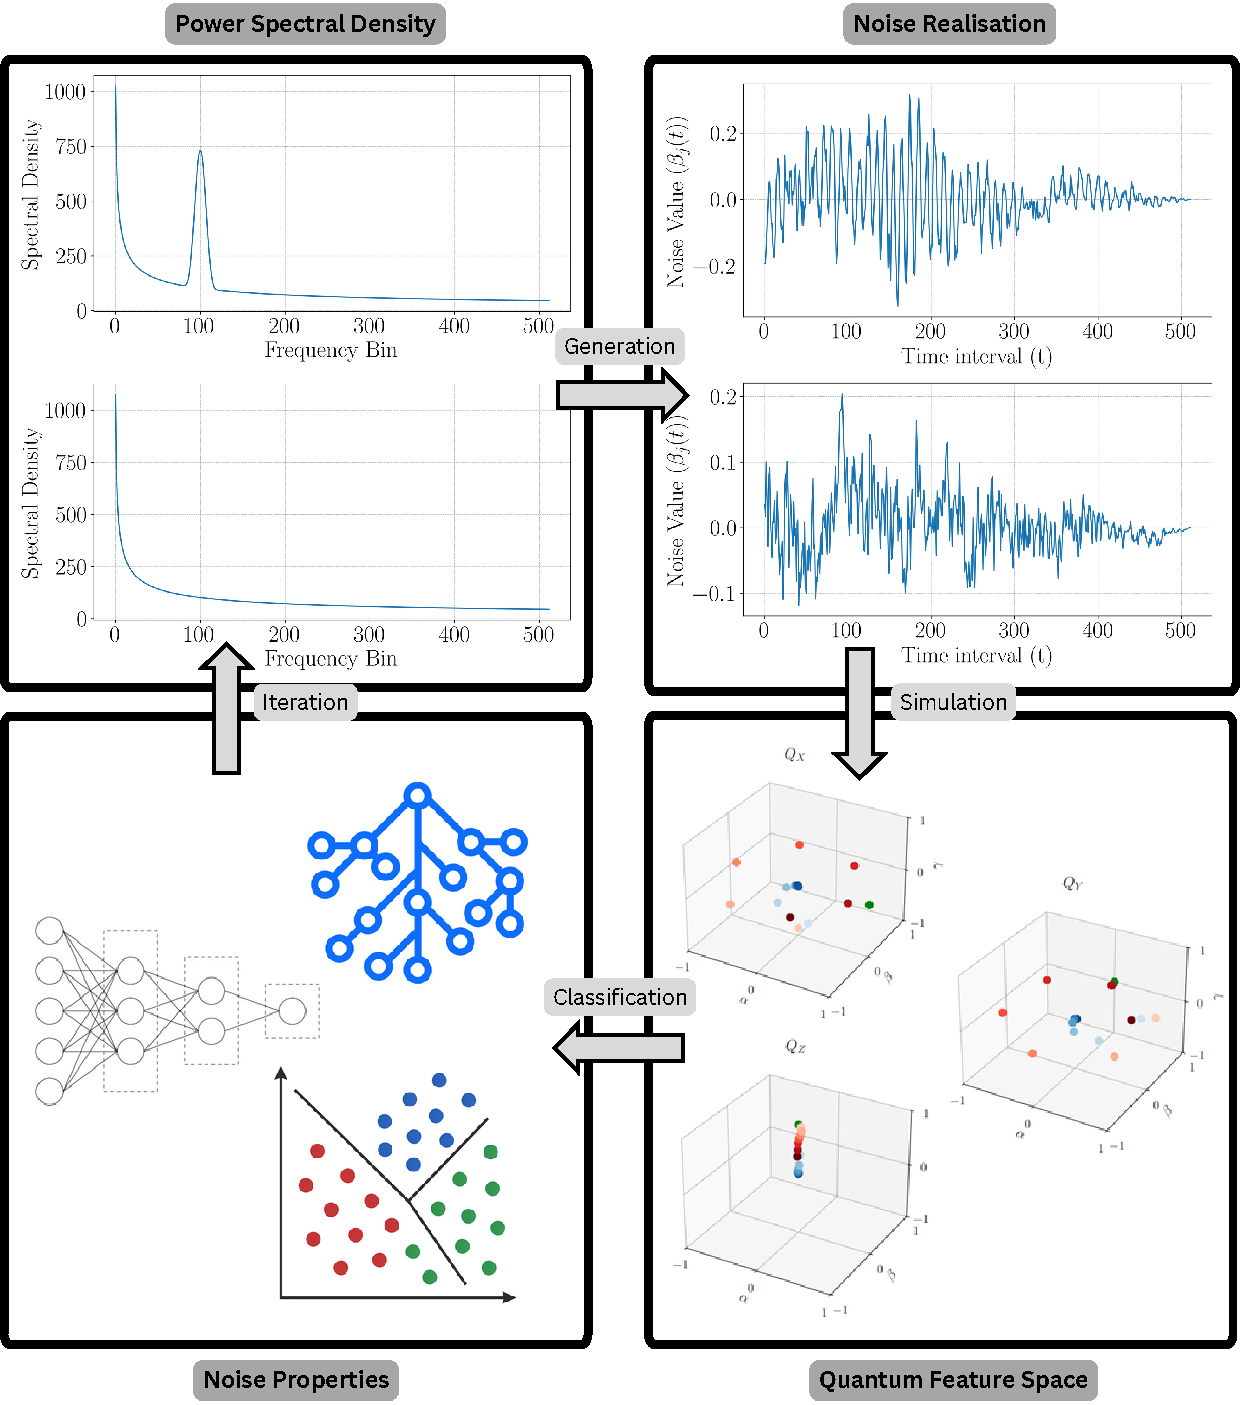
\includegraphics[width=0.7\textwidth]{figures/schematic.pdf}
    \caption{The diagram illustrates an iterative process for characterising and learning noise properties in quantum systems. Starting with a power spectral density (PSD) (top), noise realisations are generated (right) and combined with control pulses in a quantum simulation. The outcomes of these simulations are mapped onto a quantum feature space (bottom), where data points encode the effects of the noise. This feature space is used by regression models such as decision trees to infer key noise properties, including type and stationarity (left). These inferred properties refine the inferred PSD model used in subsequent iterations. This closed-loop framework enables the classification and clustering of noise processes. It facilitates tailored noise mitigation strategies, leveraging machine learning techniques like decision trees, k-means clustering, and neural networks for enhanced quantum control.}
    \label{fig:schematic}
\end{figure}

\section{Theoretical Results \label{sec:noise_operator_formalism}}
\subsection{Separating Control Dynamics From System-Bath Interaction Dynamics \label{subsec:separating_control_dynamics_from_system_environment_interaction_dynamics}}
The Hamiltonian describing a controlled qubit (the system) interacting with a bath is,
\begin{equation}
    \label{eq:total_hamiltonian}
    H(t) = H_{ctrl}(t) + H_{SB}(t)
\end{equation}
where the control Hamiltonian is,
\begin{equation}
    \label{eq:control_hamiltonian}
    H_{\mathrm{ctrl}}(t)=\Omega \frac{\sigma_{z}}{2}+\sum_{j=\{x, y, z\}} f_{j}(t) \frac{\sigma_{j}}{2}
\end{equation}
where $\Omega$ is the qubit's energy gap and $f_j(t)$ is a control pulse along the given axis, and the system-bath Hamiltonian is,
\begin{equation}
    \label{eq:system_bath_hamiltonian}
    H_{SB}(t) = \sum_{j=x, y, z} \sigma_{j} \otimes B_{j}(t)
\end{equation}
with $B_{j}(t)=\hat{B}_{j}(t)+\beta_{j}(t) I_{B}$ capturing a quantum bath via the operator $\hat{B}_{j}(t)$ and classical noise via the stochastic process $\beta_{j}(t)$.

We are interested in the expected value of a system (qubit) observable $O$ at time $T$ given an initial system (qubit) state $\rho$, where $T$ represents the total time of the control pulse sequence. This is given by,
\begin{equation} \label{eq:initial_expectation}
    \mathbb{E}\{O(T)\}_{\rho}=\left\langle\mathrm{Tr}\left[U(T)\left(\rho \otimes \rho_{B}\right) U(T)^{\dagger} O\right]\right\rangle
\end{equation}
where $U(T)=\mathcal{T} e^{-i \int_{0}^{T} H(s) \, ds}$ is the time-ordered exponential of the time-dependent Hamiltonian in~\cref{eq:total_hamiltonian}, $\langle\cdot\rangle$ denotes classical averaging over the random processes $\beta_{j}(t)$, and $\rho_{B}$ is the initial state of the bath.

We then decompose the total system-bath evolution into a product of system-bath dynamics and control dynamics. To do this, Paz-Silva, Norris, and Lorenza~\cite{paz2017multiqubit} used a so-called \textit{toggling frame}, defined by the time-ordered control unitary,
\begin{equation} \label{eq:control_unitary_construction}
    U_{\mathrm{ctrl}}(t)=\mathcal{T} e^{-i \int_0^t H_{\mathrm{ctrl}}(s) \, ds}
\end{equation}
The system-bath Hamiltonian in this toggling frame is,
\begin{equation}\label{eq:interaction_hamiltonian}
    H_{\mathrm{SB}}^{\mathrm{tog}}(t) = U_{\mathrm{ctrl}}^{\dagger}(t) H_{\mathrm{SB}}(t) U_{\mathrm{ctrl}}(t)
\end{equation}
with the associated unitary,
\begin{equation}\label{eq:interaction_unitary}
    U_{\mathrm{SB}}^{\mathrm{tog}}(t)=\mathcal{T} e^{-i \int_0^t H_{\mathrm{SB}}^{\mathrm{tog}}(s) \, ds}
\end{equation}
It can be shown that,
\begin{equation}\label{eq:final_interaction_unitary}
    {U}_{\mathrm{SB}}(t)=U_{\mathrm{ctrl}}(t)  U_{\mathrm{SB}}^{\mathrm{tog}}(t) U_{\mathrm{ctrl}}^{\dagger}(t)
\end{equation}
which allows us to rewrite~\cref{eq:initial_expectation} as,
\begin{equation} \label{eq:expectation_with_noise}
    \mathbb{E}\{O(T)\}_\rho=\mathrm{Tr}\left[V_O(T) U_{\mathrm{ctrl}}(T) \rho U_{\mathrm{ctrl}}(T)^{\dagger} O\right]
\end{equation}
where
\begin{equation} \label{eq:VO_construction}
    V_{O}(T)=\left\langle O^{-1} {U}_{\mathrm{SB}}^{\dagger}(T) O {U}_{\mathrm{SB}}(T)\right\rangle_{B}
\end{equation}
with $\left\langle \cdot \right\rangle_{B}=\left\langle\mathrm{Tr}_{B}\left[\cdot \rho_{B}\right]\right\rangle$ representing classical averaging over the partial trace taken with respect to the bath. Physically, we interpret $V_{O}$ as a so-called \textit{noise operator} that encodes the influence of the system-bath interaction on the qubit dynamics.

\subsection{Decomposition of the System-Bath Operator \label{subsec:decomposition_of_vo}}
When our system-bath Hamiltonian consists of only classical noise processes, one can move $O^{-1}$ in~\cref{eq:VO_construction}, and write,
\begin{equation} \label{eq:VO_construction_1}
    V_O=O^{-1}\left\langle U_{\mathrm{SB}}^{\dagger} O U_{\mathrm{SB}}\right\rangle
\end{equation}
where the time argument $T$ has been omitted for brevity. Before continuing, it is important to note some of the mathematical properties of the $V_O$ operator as they subsequently inform restrictions on its parameterisation. Specifically, $\left\langle U_{\mathrm{SB}}^{\dagger} O U_{\mathrm{SB}}\right\rangle$ is trace bounded by one, is Hermitian, and has real eigenvalues between $-1$ and $1$~\cite{youssry2020characterization}.

% One could parameterise $V_O$ as a general complex matrix. However, a given prediction of a complex matrix by a trained model would likely not satisfy the above properties. Further, it requires $2n^2$ (where $n$ is the matrix dimension) free parameters to be predicted. Thus, one is motivated to find a more efficient parameterisation of $V_O$.

An efficient parameterisation of $V_O$ is provided by its eigendecomposition. This eigendecomposition contains a diagonal matrix $D_O$ whose entries are real numbers in the interval $[-1, 1]$ and whose sum also lies in the interval $[-1, 1]$, and a general unitary matrix $Q$. Thus~\cref{eq:VO_construction_1} can be rewritten as
\begin{equation} \label{eq:VO_construction_2}
    V_{O} = O^{-1}Q_{O}D_{O}Q_{O}^{\dagger}
\end{equation}
In the case of a qubit, we start with a factorisation of a general $2 \times 2$ unitary operator,
\begin{equation} \label{eq:Q_construction}
    Q_{O}=\left[ \begin{array}{cc}
            e^{i \psi_O} & 0             \\
            0            & e^{-i \psi_O}
        \end{array} \right]
    \left[ \begin{array}{cc}
            \cos \theta_O  & \sin \theta_O \\
            -\sin \theta_O & \cos \theta_O
        \end{array} \right]
    \left[ \begin{array}{cc}
            e^{i \Delta_O} & 0               \\
            0              & e^{-i \Delta_O}
        \end{array} \right]\
\end{equation}
where $\psi_O, \theta_O, \Delta_O \in \mathbb{R}$ and the diagonal matrix $D_O$ of~\cref{eq:VO_construction_2} is constructed as
\begin{equation} \label{eq:D_construction}
    D_{O}=\left[ \begin{array}{cc}
            \mu_O & 0      \\
            0     & -\mu_O
        \end{array} \right]
\end{equation}
where $\mu_O \in [0,1]$. The matrix $D_O$ can be generalised to non-unital channels~\cite{youssry2020characterization}, but this paper will focus on unital channels. An unital channel is a quantum channel that maps the identity operator to the identity operator, and a non-unital channel does not~\cite{nielsen2002quantum}.

\subsection{Deriving the Quantum Feature Space \label{subsec:deducing_noise_operators}}
The previous grey-box approach to qubit control of~\cite{youssry2020characterization,youssry2022multi} used expectations and control pulse amplitudes to train a model, both classical feature spaces. This motivated us to develop a method to deduce the $V_O$ operators and their parameters from observable expectations. This allowed us to understand the properties of the qubit bath over time. The $V_O$ matrices are quantum operators, where it was hypothesised that the feature space formed from these operators' parameters is richer than those used in previous work. By creating a rich feature space, we could classify noise processes without needing expensive deep-learning models.

Substituting~\cref{eq:VO_construction_2} into~\cref{eq:expectation_with_noise} gives,
\begin{equation}
    \label{eq:expectationWithNoise3}
    \mathbb{E}\{O(T)\}_\rho = \mathrm{Tr}\left[Q_{O}D_{O}Q_{O}^{\dagger} U_{\mathrm{ctrl}} \rho U_{\mathrm{ctrl}}^{\dagger}\right]
\end{equation}

To calculate the mapping between expectations and $V_{O}$ operators, one must understand \textit{a priori} the generalised structure of $Q_{O}D_{O}Q_{O}^{\dagger}$. Recalling the definition of $Q_O$, we find $ Q_{O}D_{O}Q_{O}^{\dagger}$ is,
\begin{equation}
    \left[ \begin{array}{cc}
            \mu_O\cos(2\theta_O)
             &
            -e^{2i\psi_O}\mu_O\sin(2\theta_O)
            \\
            -e^{-2i\psi_O}\mu_O\sin(2\theta_O)
             &
            -\mu_O\cos(2\theta_O)
        \end{array} \right] = \left[ \begin{array}{cc}
            \gamma_O             & \alpha_O - \beta_O i \\
            \alpha_O + \beta_O i & -\gamma_O
        \end{array} \right]   \label{eq:QDQDagger}
\end{equation}
Now $U_{\mathrm{ctrl}} \rho U_{\mathrm{ctrl}}^{\dagger}$ must be Hermitian, with trace one, such that,
\begin{equation}
    U_{\mathrm{ctrl}} \rho U_{\mathrm{ctrl}}^{\dagger} = \left[\begin{array}{cc}
            a_{\rho}             & b_{\rho} - c_{\rho}i \\
            b_{\rho} + c_{\rho}i & 1 - a_{\rho}
        \end{array}\right] \label{eq:uctrl_rho_uctrl_dag}
\end{equation}
with $0 \leq a_{\rho} \leq 1$.

We can now calculate the generalised form of $\mathbb{E}\{O(T)\}_\rho$ in terms of the newly introduced parameters,
\begin{equation}
    \mathbb{E}\{O(T)\}_\rho = 2 b_{\rho} \alpha_{O}  + 2 c_{\rho} \beta_{O} + (2a_{\rho} - 1)\gamma_{O} \label{eq:expectation_as_function_of_parameters}
\end{equation}

For each observable, there are six initial states, so to find solutions $\alpha_{O}, \beta_{O}, \gamma_{O}$ for each observable, we need to solve an over-determined system of six equations with three unknowns,
\begin{equation} \label{eq:overdetermined-full-definition}
    \left[\begin{array}{ccc}
            2b_{\rho_{x_+}} & 2c_{\rho_{x_+}} & (2a_{\rho_{x_+}} - 1) \\
            2b_{\rho_{x_-}} & 2c_{\rho_{x_-}} & (2a_{\rho_{x_+}} - 1) \\
            \vdots          & \vdots          & \vdots                \\
            2b_{\rho_{z_-}} & 2c_{\rho_{z_-}} & (2a_{\rho_{z_-}} - 1) \\
        \end{array}\right]
    \left[\begin{array}{c}
            \alpha_{O} \\
            \beta _{O} \\
            \gamma_{O} \\
        \end{array}\right]
    =
    \left[\begin{array}{c}
            \mathbb{E}\{O\}_{\rho_{x_+}} \\
            \mathbb{E}\{O\}_{\rho_{x_-}} \\
            \vdots                       \\
            \mathbb{E}\{O\}_{\rho_{z_-}}
        \end{array}\right]
\end{equation}
with $\rho_{x_+}, \rho_{x_-}, \ldots, \rho_{z_-}$ being the standard eigenstates of the Pauli matrices.

% Evaluating the eigenvalues of the parameterisation of $Q_{O}D_{O}Q_{O}^{\dagger}$ in~\cref {eq:QDQDagger} yields
% \begin{equation}
%     \mu_O = \sqrt{\gamma_O^2 + \alpha_O^2 + \beta_O^2}
% \end{equation}
% where $0 \leq \mu_O \leq 1$. Equating the parameterised forms of $Q_{O}D_{O}Q_{O}^{\dagger}$ we find,
% \begin{equation}
%     \theta_O = \frac{1}{2}\arccos\left(\frac{\gamma_O}{\mu_O}\right) \label{eq:theta_calculation}
% \end{equation}
% \begin{equation}
%     \psi_O = \frac{1}{2} \mathrm{Im}\left[\ln\left(\frac{\alpha_O + \beta_O i}{\mu_O\sin(2\theta_O)}\right)\right] \label{eq:psi_calculation}
% \end{equation}
% where $0 \leq \theta_O \leq \frac{\pi}{2}$, and $-\frac{\pi}{2} \leq \psi_O < \frac{\pi}{2} $.

This section has shown that the parameters $\alpha_O$, $\beta_O$, and $\gamma_O$ can be deduced from observable expectations, where such parameters form the quantum feature space.
\section{Experimental Results \label{sec:visulisation_of_noise_operator_parameters}}
\subsection{Efficiency of Quantum Feature Space Derivation \label{sec:quantum_feature_space_derivation_efficiency}}
To find the best-fit solution of~\cref{eq:overdetermined-full-definition}, we used the Moore-Penrose inverse~\cite{penrose1955generalized}. We implemented the Moore-Penrose inverse and methodologies of~\cref{subsec:deducing_noise_operators} using \textit{Pytorch}~\cite{paszke2019pytorch} and parallelised calculations using a GPU. The GPU for all experiments and simulations was an NVIDIA GeForce RTX 3060 with 12GB of memory.

To test and verify the methods of~\cref{subsec:deducing_noise_operators} we used ground truth expectations and the corresponding $V_O$ operators from \textit{QDataSet}~\cite{perrier2022qdataset}. A batch of 1000 expectations was used to derive the parameters $\mu_O$, $\theta_O$, and $\psi_O$, with a total time taken of $0.52 \pm 0.05$ms.
\subsection{Quantum Simulation Implementation \label{subsec:quantum_simulation_implementation}}
We noted inefficiencies in the simulator of~\cite{perrier2022qdataset}, which led to long execution times. Our redesigned simulator addressed these issues while making it more adapted to other related tasks.

A major improvement was using tensor operations whenever possible for the operations presented in~\cref{sec:noise_operator_formalism}. In our implementation when computing the unitary at timestep $t$, this was done by left multiplying the unitary at time step $t-1$ by the exponentiated Hamiltonian at time step $t$. This method was not used in the previous simulator to compute unitaries, and instead, unitaries were computed via recomputing the entire product of required exponentiated Hamiltonians.

A further improvement was that our simulation did not compute the interaction unitaries for all timesteps; instead, only the final time step interaction unitary was calculated as this was the only interaction unitary required for expectation calculations. By enforcing this, we could exploit the associativity of matrix multiplication and implement a binary tree structure to compute the final unitary, which required $O(\log(N))$ multiplications, where $N$ is the number of time steps.

We benched marked our simulator and found what required a few days for single qubit simulations in the previous implementation~\cite{perrier2022qdataset} took 10 minutes with the new simulator, giving over a 400$\times$~improvement. Greater speed-ups can be achieved if computing at lower precision and or using a GPU with more memory, where both options enable larger batch sizes.

\subsection{Creation of Quantum Feature Space Data \label{subsec:creation_of_quantum_feature_space_data}}
To create the quantum feature space data, we started with noise models and realisation generation methods following that of \textit{QDataSet}~\cite{perrier2022qdataset}. All noise processes acted along the $x$ and $z$ axes, with the noise processes being correlated between the axes. This correlation was achieved by setting the noise values along the $z$-axis to be the absolute value of the $x$-axis values (similar to noise profile N6 in \textit{QDataSet}).

Our experiments explored the following noise processes:
\begin{itemize}
    \item a noise process with a $1/f$ noise power spectral density (PSD) (N5 in \textit{QDataSet})
    \item a noise process with a $1/f$ noise PSD with a Gaussian bump in the PSD (N1 in \textit{QDataSet})
    \item a Gaussian coloured noise process (N2 in \textit{QDataSet})
\end{itemize}
There were six different noise processes in total. The first three were the above noise processes, and the other three were non-stationarity variants of each noise process. To achieve non-stationarity, we multiplied the noise processes by a deterministic triangular time envelope. The envelope was a triangular function with a peak at $T/2$ and a width of $T$.

The second noise process ($1/f$ with a bump) was chosen because it shared similarities with the first noise process ($1/f$). It was hypothesised that these two noise processes would result in parameters close together in the quantum feature space. Conversely, the third (stationary coloured) was chosen because it was hypothesised that it would result in parameters far from the points of the first two noise processes.

Control pulses were applied along the $x$-axis for all simulations, where the control pulses were approximations of CPMG pulses. To achieve CPMG pulses, we created Gaussia-shaped pulses of the form
\begin{equation} \label{eq:gaussian_pulse}
    f_{j}(t)=\sum_{n=1}^{n_{\max }} A_n e^{-\frac{\left(t-\tau_{n}\right)^{2}}{2 \sigma^{2}}}
\end{equation}
where $\sigma=\frac{T}{\lambda M}$, $\lambda \in \mathbb{R}^+$ is the pulse width, $T$ is the total time, $M$ is the number of time steps, $\tau_{n}=\left(\frac{n-0.5}{n_{\max }}\right) T+\delta_{\tau}$, with $\delta_{\tau} \in \mathbb{R}$ being used to add jitter to the pulse timing, and $A_n$ is the amplitude of the $n^{\mathrm{th}}$ pulse.

For all experiments $n_{\max}=5$, 1024 discrete time steps were used and, ensemble averaging was performed over 2000 realisations of the noise process for a given control pulse sequence.

\subsection{Black Box Classification of Bath Through Quantum Feature Space \label{subsec:black_box_noise_spectroscopy}}
We conducted a series of simulations to test the ability of the quantum feature space to classify distinct noise processes, where the quantum feature space ($Q_O$) is the space formed by using the three parameters $\alpha_O$, $\beta_O$, and $\gamma_O$ from~\cref{eq:QDQDagger}.

We first simulated qubit dynamics subject to realisations of the above noise processes with the approximated ideal CPMG pulses. We then simulated a $1/f$ noise process with a bump in the PSD, changing the location of its peak compared to earlier noise processes, which acted as an unknown noise process from a physical experiment that an experimentalist would be trying to classify.

While simulating a qubit in the presence of the realisation of an unknown noise process, we used more realistic CPMG pulses; the pulse width was increased, and jitter was added to the peak's timing and value. From the realistic CPMG pulses, we ended up with a cluster of points in feature space arising from distinct realisations of the jitter. In a black box manner, we identify which noise process characterises the unknown noise process by measuring which \textit{a priori} noise process the cluster of points was closest to in the quantum feature space.

To simulate ideal CPMG pulses, we set $\lambda = \frac{1}{96}$, $\delta_{\tau} = 0$, $n_{\max} = 5$, and $A_n = \pi$. These values were chosen to approximate delta function pulses (See~\cref{fig:control_pulses_visualisation} top row).

To simulate the realistic CPMG pulses we set $\lambda = \frac{1}{24}$, $\delta_{\tau}$ was chosen from a uniform random distribution spanning the interval $[-\frac{24T}{M}, \frac{24T}{M}]$, and $A_n = \pi + \epsilon$ where $\epsilon$ was drawn from a uniform random distribution spanning the interval $[-\frac{\pi}{5}, \frac{\pi}{5}]$ (See~\cref{fig:control_pulses_visualisation} bottom row). 50 such unique realistic control pulse sequences were generated with ensemble averaging over 2000 noise process realisations for each control pulse, resulting in a cluster of 50 unique points in the quantum feature space.

\begin{figure}
    \centering
    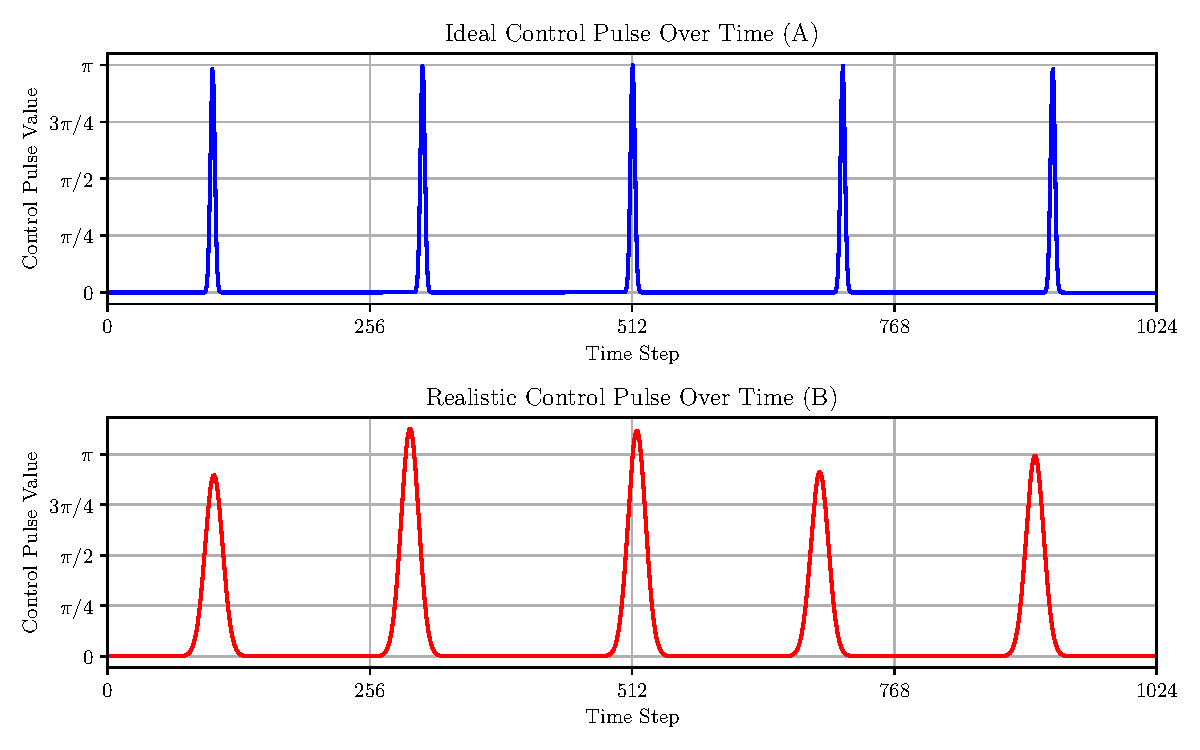
\includegraphics[width=\textwidth]{figures/control_pulses.pdf}
    \caption{Control pulses used in the simulations. The top row shows the ideal CPMG pulses and the bottom row shows the realistic CPMG pulses.}
    \label{fig:control_pulses_visualisation}
\end{figure}

From the first round of simulations, we calculated the average of the Euclidean distances between the realistic data points and the single data point from the \textit{a priori} noise processes for the feature spaces associated with \(Q_X\), \(Q_Y\), and \(Q_Z\). We found that the `$1/f$ + bump' noise process had the smallest total average Euclidean distance across all feature spaces, indicating the unknown noise process is likely closest to the unknown noise process.

To refine our estimate of the unknown noise process, using the first round's results, we simulated several `$1/f$ + bump' noise profiles, varying the location of the peak in the PSD. Specifically, peaks were positioned at predefined frequency bins, such as the 15th or 30th bin. The results indicated that the noise processes with peaks in the $240^\mathrm{th}$ and $120^\mathrm{th}$ bins were the closest matches, as measured by the average Euclidean distances in the quantum feature space to the unknown process, which peaks at the $200^\mathrm{th}$ bin.

\begin{table}[ht]
    \centering
    \begin{tabular}{lcccccc}
        \toprule
              & $1/f$          & $1/f$ (NS)     & $1/f$ + bump   & $1/f$ + bump (NS) & Coloured & Coloured (NS) \\
        \midrule
        $V_x$ & 0.398          & \textbf{0.368} & 0.379          & 0.381             & 0.828    & 0.924         \\
        $V_y$ & 0.303          & 0.307          & \textbf{0.246} & 0.269             & 0.812    & 0.857         \\
        $V_z$ & \textbf{0.290} & 0.297          & 0.304          & 0.293             & 0.687    & 0.621         \\
        \midrule
        Total & 0.991          & 0.973          & \textbf{0.929} & 0.943             & 2.326    & 2.402         \\
        \bottomrule
    \end{tabular}
    \caption{Average Euclidean distances between realistic data points and the corresponding noise process values in the feature spaces of \(Q_X\), \(Q_Y\), and \(Q_Z\). For each \(V_O\) (row), the lowest (best) value is bolded. The total distance is the sum of the distances across all three feature spaces. The overall closest noise process is the `$1/f$ + bump' noise process, with the smallest total distance as bolded.}
    \label{tab:noise_profiles}
\end{table}

\begin{table}[ht]
    \centering
    \begin{tabular}{lcccccc}
        \toprule
              & $15^\mathrm{th}$ & $30^\mathrm{th}$ & $60^\mathrm{th}$ & $120^\mathrm{th}$ & $240^\mathrm{th}$ & $480^\mathrm{th}$ \\
        \midrule
        $V_x$ & 0.367            & 0.365            & 0.367            & 0.322             & \textbf{0.279}    & 0.557             \\
        $V_y$ & 0.241            & 0.239            & 0.226            & 0.153             & \textbf{0.108}    & 0.578             \\
        $V_z$ & 0.296            & 0.282            & 0.303            & 0.292             & \textbf{0.279}    & 0.286             \\
        \midrule
        Total & 0.903            & 0.885            & 0.896            & 0.767             & \textbf{0.666}    & 1.422             \\
        \bottomrule
    \end{tabular}
    \caption{Average Euclidean distances between realistic data points and the corresponding noise process values in the feature spaces of \(Q_X\), \(Q_Y\), and \(Q_Z\). For each \(V_O\) (row), the lowest (best) value is bolded. The total distance is the sum of the distances across all three feature spaces. The overall closest noise process is the $240^\mathrm{th}$ noise profile, as indicated by the lowest total distance.}
    \label{tab:noise_profiles_new}
\end{table}

It is interesting to note the significantly larger distances between the `$1/f$ + bump' noise processes and the coloured noise processes. This enforces the hypothesis that the quantum feature space encodes the noise process characteristics, as such all the coloured noise processes are significantly further away from the `$1/f$ + bump' noise processes than the `$1/f$ + bump' noise processes are from each other. On the other hand, each noise process has a similar distance metric to its corresponding non-stationary noise process. This indicates that the non-stationary and stationary noise processes result in similar parameters in the quantum feature space, indicating that the quantum feature space is not as sensitive to non-stationarity.

Further, for the second round of simulations, we see that as the peak location in the PSD moves further away from the $200^\mathrm{th}$ bin, the average Euclidean distance increases. Further strengthening the hypothesis that the quantum feature space encodes the noise process characteristics and distances in noise characteristics (i.e. the distance between PSD peaks) manifest themselves as distances in the quantum feature space.

The result in this section demonstrates that one could simulate a broad class of noise processes to derive quantum features and compare them to quantum features from experimental data with an unknown noise process. Once the general noise process is found, a binary search could be performed to estimate specific parameters of this unknown noise process by minimising distance in the quantum feature space.

\subsection{Decision Tree for Noise Characterisation \label{subsec:decision_tree_for_noise_characterisation}}
We then explored the ability of simple ML algorithms to use this quantum feature space. To do this, we generated 600 different noise processes and trained a random forest with K-Fold cross-validation~\cite{james2013introduction, scikit-learn}.

For the 600 distinct noise processes, 200 processes were $1/f$, 200 were $1/f$ with a bump, and 200 were coloured noise. For each noise process class, half were stationarity, and half were non-stationary, i.e. 100 $1/f$ stationary noise processes and 100 $1/f$ non-stationary noise processes. We randomised several parameters between each noise profile to create distinct processes to ensure a diverse and representative dataset.~\cref{tab:noise_profiles} summarises the randomised parameters for each noise process and the range of values used. For the $1/f$ noise processes, the exponent ($\alpha$) was varied, and for the $1/f$ noise profiles with a bump, the bump location in the frequency domain ($\mu$) was varied alongside $\alpha$. For coloured noise, the division factor controlling the filter was randomised. For all non-stationary profiles, the peak position of the triangle envelope as a fraction of the total time ($T$) was randomised.

\begin{table}[h!]
    \centering
    \begin{tabular}{|l|l|l|}
        \hline
        \textbf{Noise Profile Type} & \textbf{Parameter}           & \textbf{Range/Value} \\ \hline
        $1/f$ Noise                 & $\alpha$                     & [0.7, 1.3]           \\ \hline
        $1/f$ Noise with Bump       & $\mu$                        & [0, 256]             \\ \cline{2-3}
                                    & $\alpha$                     & [0.7, 1.3]           \\ \hline
        Coloured Noise              & Division Factor              & [2, 16]              \\ \hline
        Non-Stationary              & Peak of deterministic signal & [0.1$T$, 0.9$T$]     \\ \hline
    \end{tabular}
    \caption{Summary of noise profile characteristics.}
    \label{tab:noise_profiles}
\end{table}

To analyse the noise profiles, we used a random forest classifier from the \textit{scikit-learn} library~\cite{scikit-learn}. The classifier was trained on the combined vector components across all three quantum feature spaces, employing a 10-fold cross-validation approach. Each sample was labelled for stationarity and noise type, where two different trees were trained for each classification task. The decision tree classifier for stationarity achieved an average test accuracy of 0.98, and the noise type classifier achieved an average test accuracy of 0.97.

The feature importances for stationarity and noise type classification are shown in~\cref{tab:feature_importances}. The feature importance is calculated as the sum of the reduction in the Gini impurity index across all nodes in the tree that use the feature~\cite{scikit-learn}. Interestingly, for both classification tasks, only 3-4 features were needed to explain the majority of the variance in the data, where at least one feature per observable had high importance. This demonstrates how noise process characteristics manifest themselves in the quantum feature space, which may assist in future work to clarify the mapping between a given noise process characteristic and the quantum feature space.

\begin{table}[h]
    \centering
    \begin{tabular}{|l|c|c c c|c c c|c c c|}
        \hline
        Classification Task & Test Accuracy & \(\alpha_X\) & \(\beta_X\) & \(\gamma_X\) & \(\alpha_Y\) & \(\beta_Y\) & \(\gamma_Y\) & \(\alpha_Z\) & \(\beta_Z\) & \(\gamma_Z\) \\ \hline
        Stationarity        & 0.98          & 0.22         & 0.08        & 0.16         & 0.08         & 0.15        & 0.03         & 0.05         & 0.08        & 0.15         \\ \hline
        Noise Type          & 0.97          & 0.09         & 0.14        & 0.07         & 0.15         & 0.13        & 0.08         & 0.03         & 0.03        & 0.28         \\ \hline
    \end{tabular}
    \caption{Average test accuracies and feature importances. Feature importances represent the average contributions of the features \(\alpha\), \(\beta\), and \(\gamma\) for each of the Quantum Feature Spaces \(Q_X\), \(Q_Y\), and \(Q_Z\) to the classification task. The feature importances are normalised to sum to 1.}
    \label{tab:feature_importances}
\end{table}

The high accuracy of a simple inexpensive ML algorithm, random forest in this case, in both tasks demonstrates the effectiveness of the quantum feature space parameters in distinguishing between different noise processes and determining their stationarity. These results further validate our approach and provide a robust method for characterising and classifying noise in quantum systems.

\subsection{Properties of the $V_O$ Parameter Space \label{subsec:properties_of_vo_parameter_space}}
We sought to understand the mapping between control and noise parameters and the quantum feature space. For these experiments, we explored the impact of widening control pulse widths, which simulated less ideal delta function pulses, the interpolation between noise profiles, and the impact of increasing noise energy.

We first explored the impact of widening control pulse widths on the quantum feature space. The control pulse width was varied by changing the value of $\lambda$ in~\cref{eq:gaussian_pulse}. We set $\lambda = \frac{1}{96}$, $\frac{1}{48}$, $\frac{1}{24}$, $\frac{1}{12}$, $\frac{1}{6}$, and $\frac{1}{3}$. For these simulations, we used the $1/f$ noise process with a bump in the PSD at the $200^\mathrm{th}$ bin, the unknown noise process from~\cref{subsec:black_box_noise_spectroscopy}.

\cref{fig:vo_space_with_changing_parameters}(a) illustrates the impact of widening control pulse widths. The figure shows the interpolation between data points arising from widening control pulses is smooth and well-ordered, supporting the quantum feature space as a well-behaved feature space, where it is known that smooth interpolation in a feature space is a highly desirable characteristic~\cite{123}

The results in~\cref{fig:vo_space_with_changing_parameters}(b) are similar and show a smooth interpolation between the $1/f$ noise process with a bump and the coloured Gaussian noise process. These interpolations were achieved by creating various linear combinations of the noise processes at different ratios, progressively transitioning from one to the other.

We then investigated the impact of increasing the signal energy of the $1/f$ with a bump and coloured Gaussian noise processes.  Signal energy here is defined as,
\begin{equation}
    \label{eq:signal_energy}
    E = \sum_{i=1}^{N} \left|n_i\right|^2
\end{equation}
where $n_i$ is the noise process value at time step $i$ and $N$ is the total number of time steps. To implement increasing energy, we scaled all values of a given noise realisation (i.e. all $n_i$) by a constant factor. Using the following scale factors: 0.25, 0.5, 0.75, 1.0, 1.25, 1.5, 1.75.

Results for increasing noise strengthen experiments are depicted in~\cref{fig:vo_space_with_changing_parameters}(c), where increasing colour saturation represents increasing energy.

For the coloured noise process, as the noise strength increases, all points tend toward the centre of the feature space, where $\alpha_O$, $\beta_O$, and $\gamma_O$ are all equal to zero.

Observe that when $\alpha_O$, $\beta_O$, and $\gamma_O = 0$, $Q_OD_OQ_O^{\dagger}$ becomes a zero matrix, and looking to~\cref{eq:expectationWithNoise3}, we find that the expectation of the observable is zero. This indicates that as the noise process increases in energy it saturates the system, and as such all information is lost. Conversely, as the noise strength decreases, points move toward the associated identity in the quantum feature space and therefore result in the system dynamics being dominated by the control pulses.

The $1/f$ + bump noise process shows a more complex behaviour in~\cref{fig:vo_space_with_changing_parameters}(c). The red dots, which represent the $1/f$ + bump noise process, appear to rotate around the $Q_X$ and $Q_Y$ axes as the noise strength increases. This rotation is likely due to the spectral bump in the noise profile, which introduces off-diagonal components into the effective noise operator.

In a quantum system under control pulses, such off-diagonal elements can lead to phase shifts or rotations in the operator representation. Essentially, the result shows that the $1/f$ + bump noise process does not simply scale the operator uniformly; it alters its orientation in the feature space.

For the $1/f$ noise process, again there is a tendency to spiral into the centre of the feature space indicating again that as the noise becomes stronger, noise saturation occurs and information is lost.

It is interesting to note that for the $1/f$ noise process, the second strongest noise point is closest to the identity (rather than the weakest noise point). One explanation of this phenomenon is the interplay between the noise's rotational effect and its contracting effect (i.e., the tendency to “wash out” information) is non-linear. As such, at a particular noise level, the destructive interference between the control dynamics and the noise perturbations may nearly cancel out.

For both noise processes, behaviour in the $Q_z$ feature space is more intuitive; points get closer to the identity as the noise decreases, indicating that the control pulses are dominating system dynamics.

Overall this nuanced behaviour seen in these experiments highlights the richness of the quantum feature space and suggests that further study—perhaps through controlled variations or analytical modeling—could provide deeper insight into these dynamics.

\begin{figure}
    \centering
    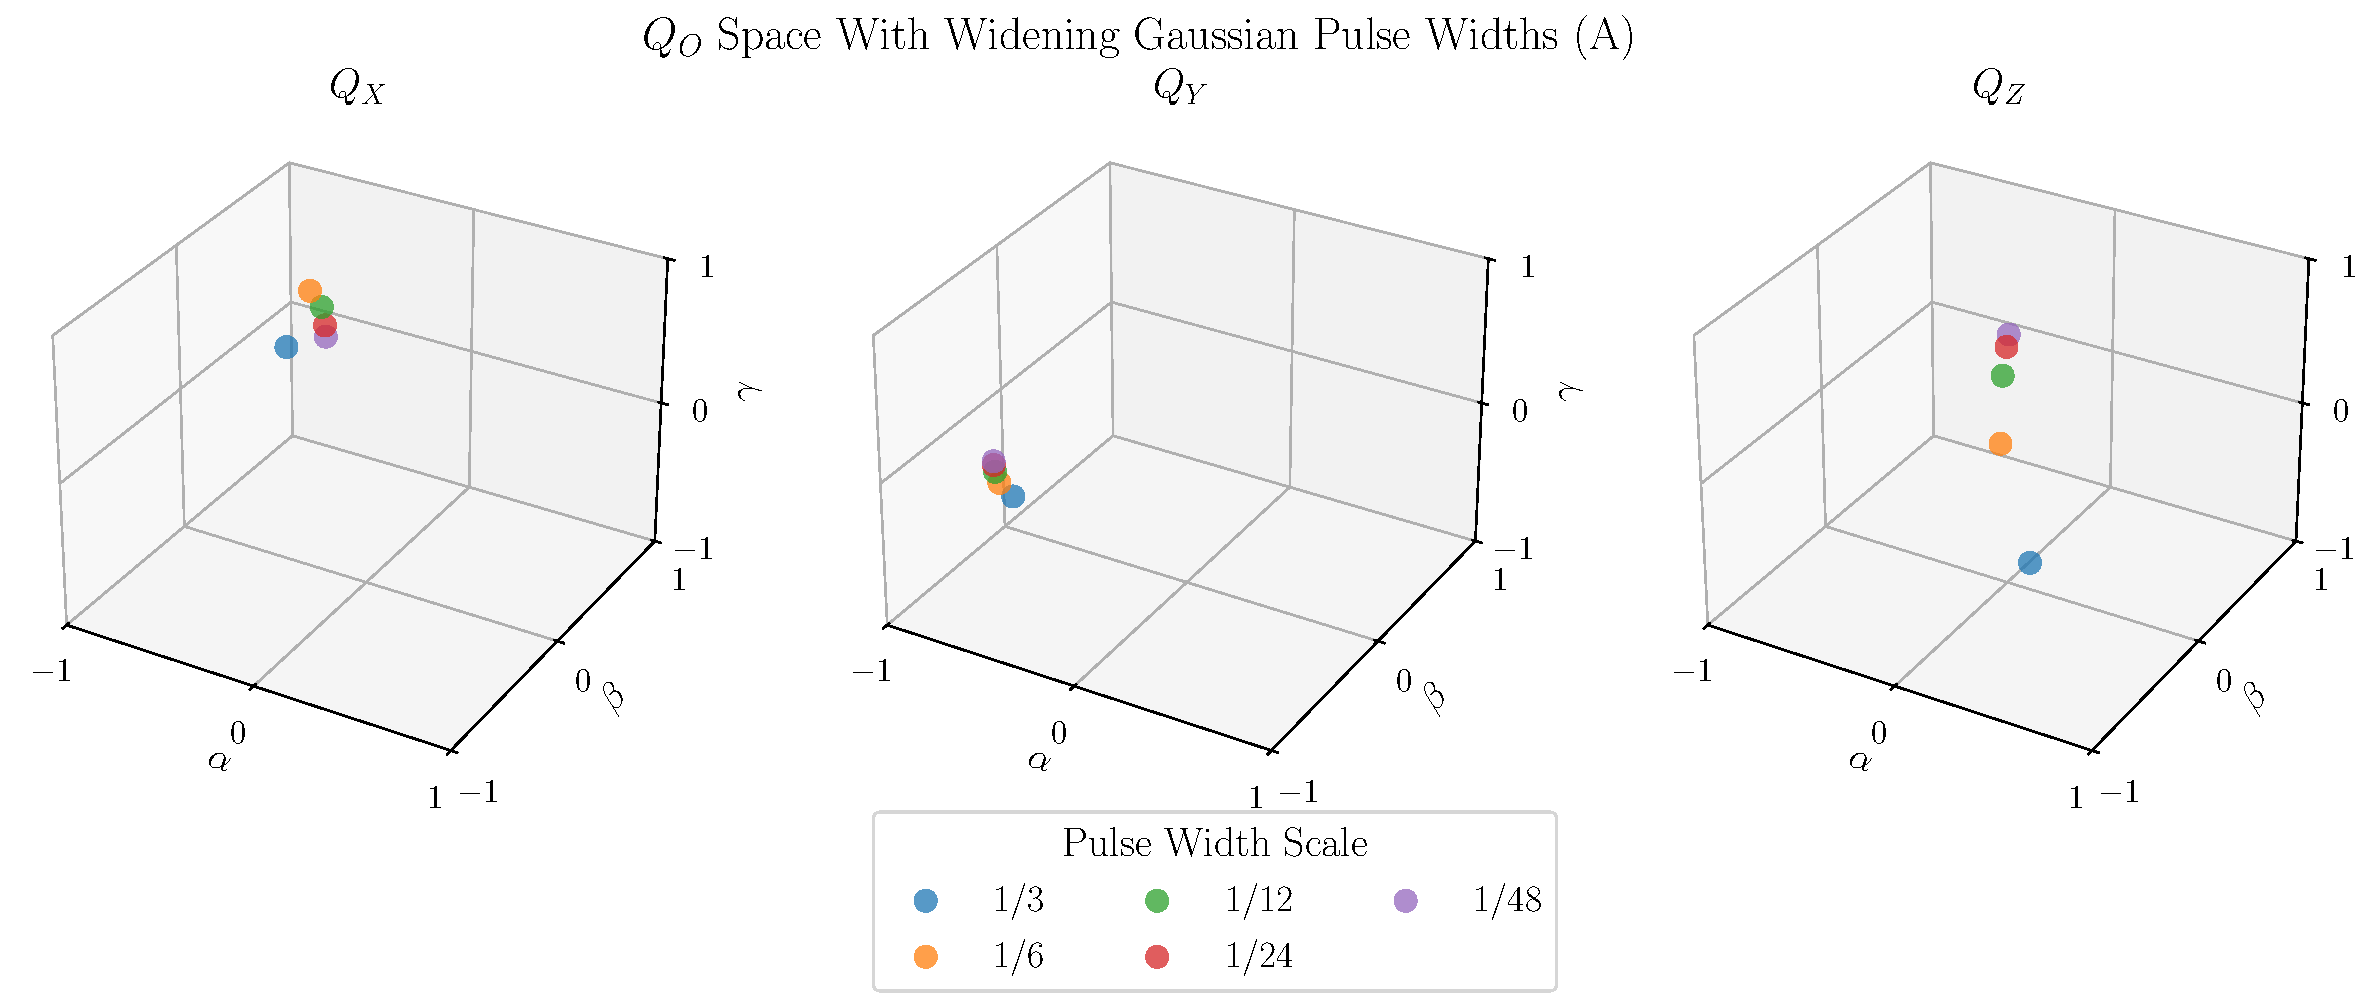
\includegraphics[width=\textwidth]{figures/vis_widening_pulses.pdf}

    \vspace{1cm}

    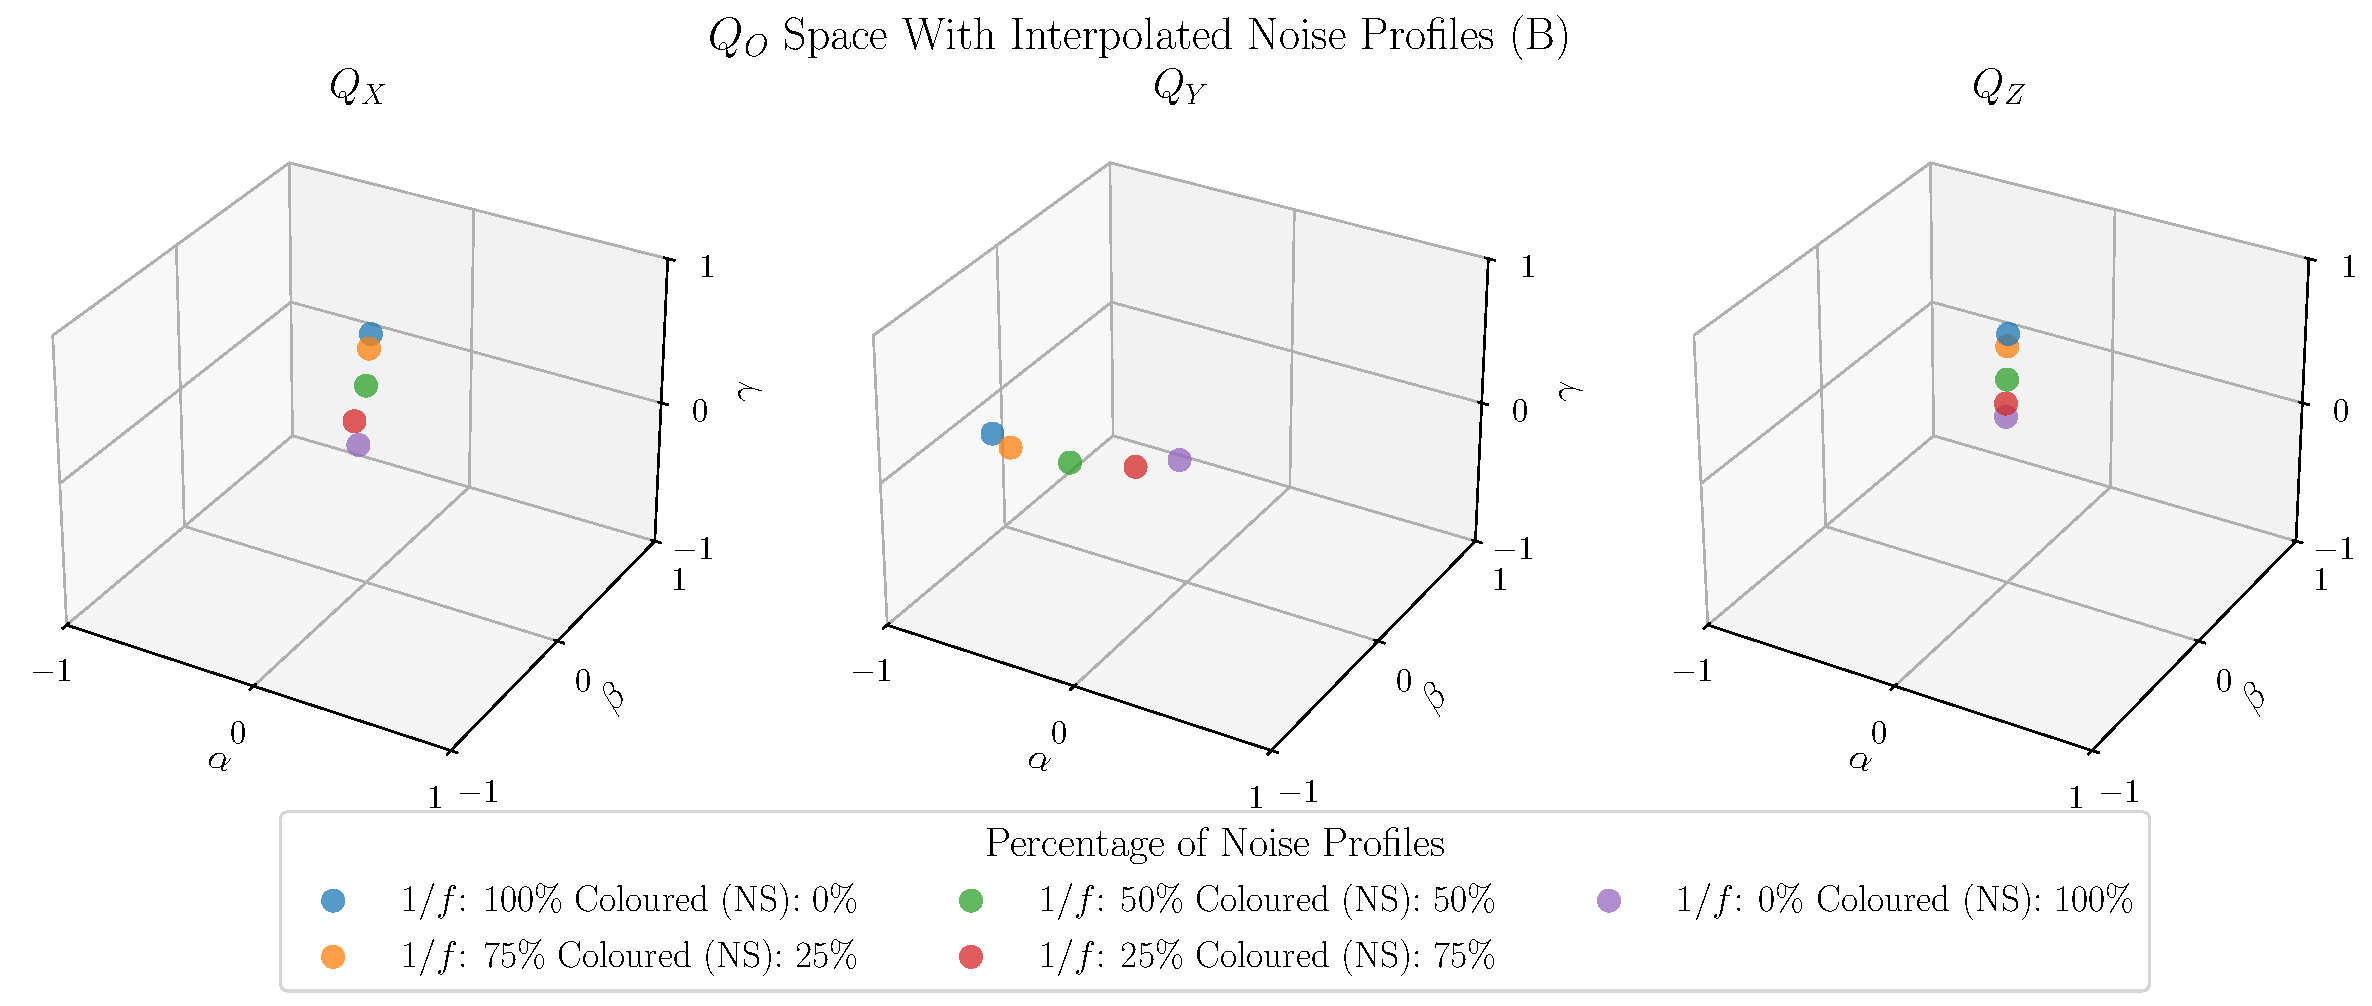
\includegraphics[width=\textwidth]{figures/vis_interpolated_noise_profiles.pdf}

    \vspace{1cm}

    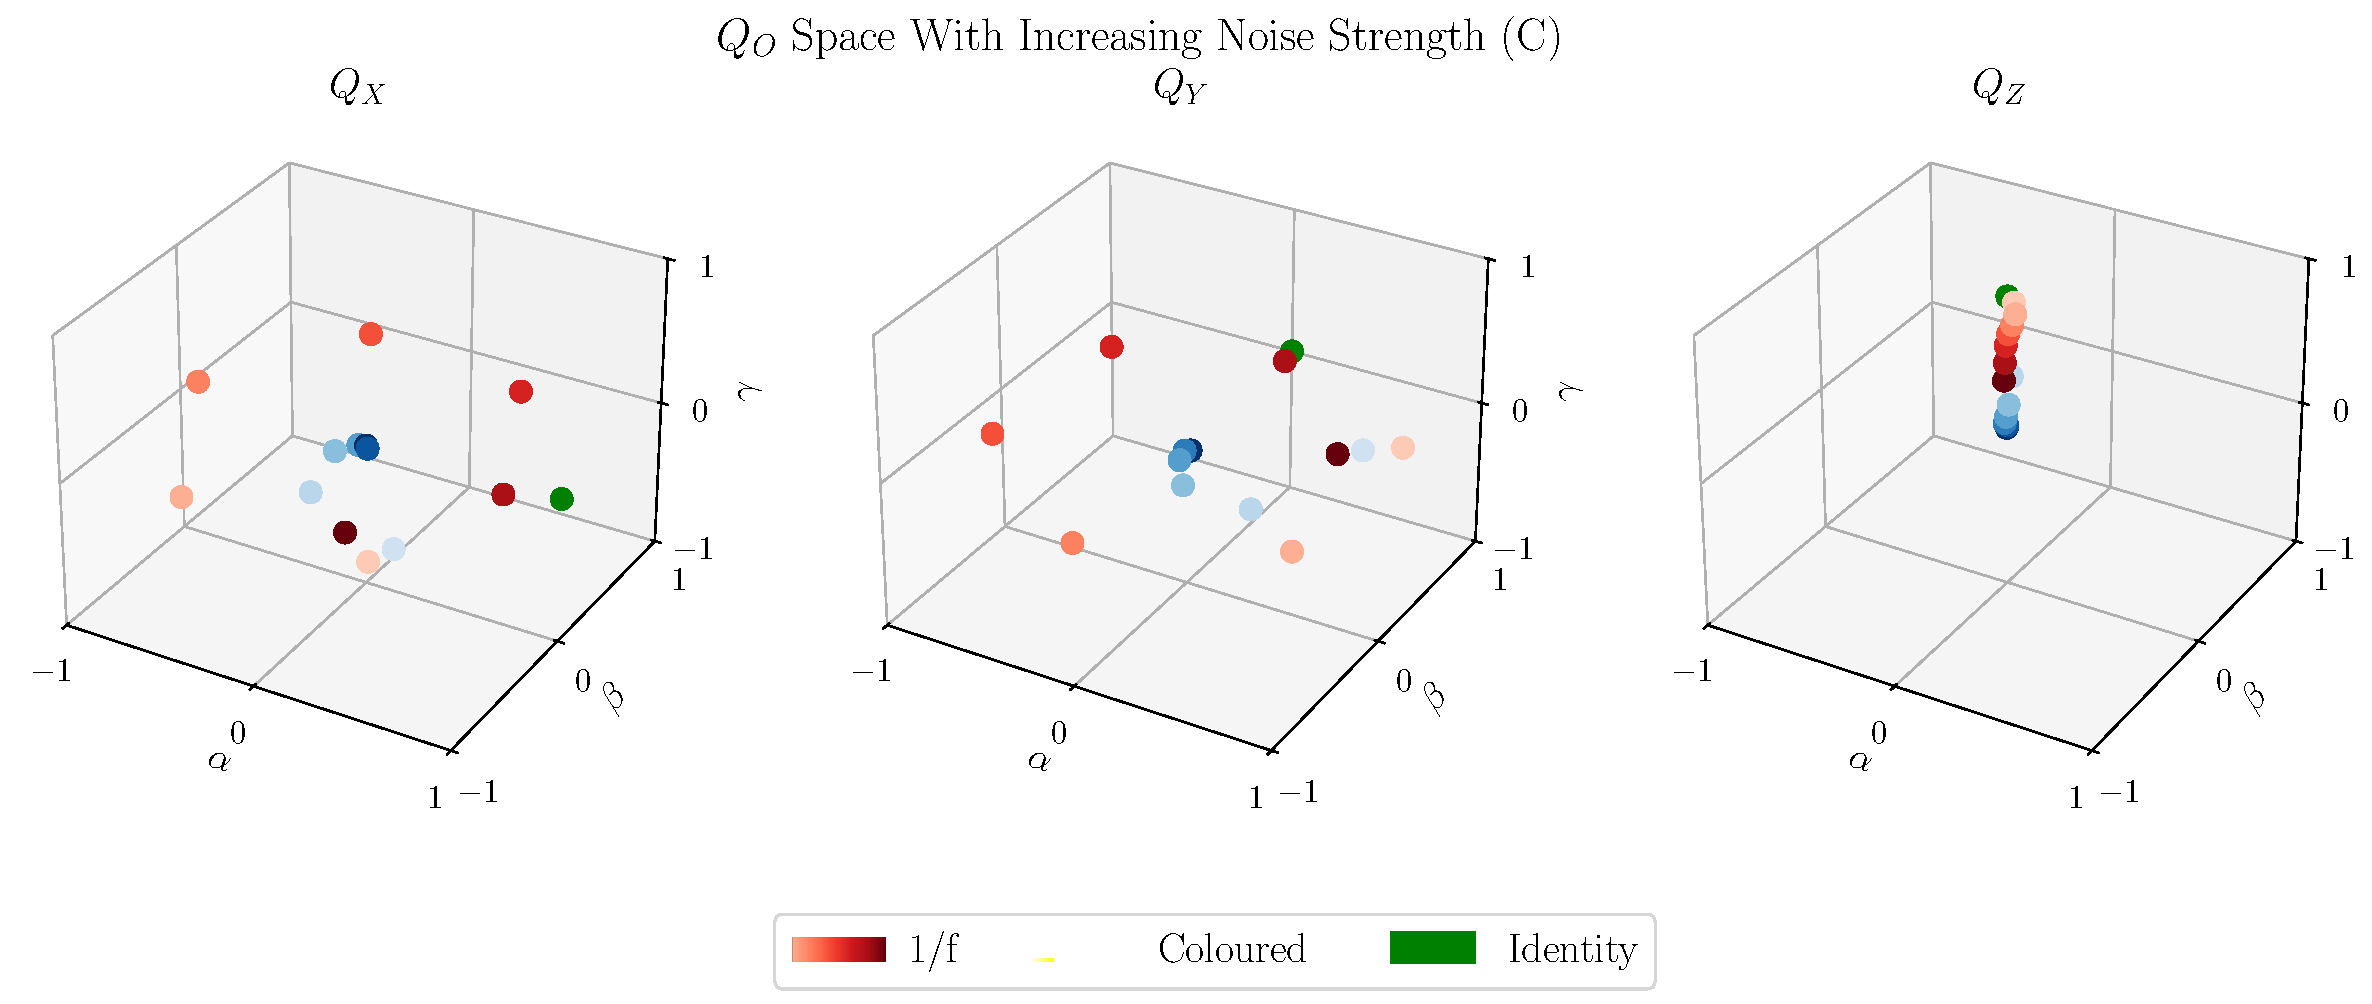
\includegraphics[width=\textwidth]{figures/vis_increasing_noise_str.pdf}
    \caption{(a) Visualisation of the quantum feature space with widening Gaussian-shaped control pulses, with fraction indicating the scale factor. (b) Visualisation of the quantum feature space with interpolation between noise processes implemented by utilising a linear combination of the $1/f$ noise process with a bump and coloured Gaussian noise process. (c) Visualisation of the quantum parameter space with two different noise processes, $1/f$ noise process with a bump and coloured Gaussian noise process, with colour saturation representing increasing energy.}
    \label{fig:vo_space_with_changing_parameters}
\end{figure}

\section{Conclusion and Future Work \label{sec:conclusion_and_future_work}}
This work has introduced a quantum feature space based on the $V_O$ noise operator formalism. To create this quantum feature space, we extended the noise operator formalism to map experimental measurements directly to system-bath interaction operator parameters. We visualised the quantum feature space, mapping its behaviour to control pulse and noise process parameters.

It was found that quantum feature spaces can be illuminating and can be used to identify unknown qubit noise processes without making restrictive assumptions. This feature space is a promising tool for future noise characterisation.

Future work could further refine control techniques within the quantum feature space, enhancing the ability to mitigate noise effects. In particular, exploring different types of control pulses and their parameters could provide deeper insights into optimising qubit control for various noise environments. Future work could include studying a broader range of noise processes to further validate the developed methodology's robustness. Incorporating non-stationary and non-Gaussian noise models further helps us understand the quantum feature space. The methods developed could also be applied to systems with more qubits in both simulated and experimental settings.

\section{Data and Code Availability \label{sec:data_and_code_availability}}
The data and code are available here:

\section*{Acknowledgments \label{sec:acknowledgments}}
Matt Woolley acknowledges support from the Australian Research Council (ARC) Centre of Excellence for Engineered Quantum Systems CE170100009. Akram Youssry acknowledges support from the Australian Research Council (ARC) Discovery Project DP210101198.

AP acknowledges an RMIT University Vice-Chancellor's Senior Research Fellowship and a Google Faculty Research Award. This work was supported by the Australian Government through the Australian Research Council under the Centre of Excellence scheme (No: CE170100012).
\section{References}
\bibliographystyle{unsrt}
\bibliography{references}

\end{document}